% Options for packages loaded elsewhere
% Options for packages loaded elsewhere
\PassOptionsToPackage{unicode}{hyperref}
\PassOptionsToPackage{hyphens}{url}
\PassOptionsToPackage{dvipsnames,svgnames,x11names}{xcolor}
%
\documentclass[
  authoryear,
  preprint,
  3p,
  onecolumn]{elsarticle}
\usepackage{xcolor}
\usepackage{amsmath,amssymb}
\setcounter{secnumdepth}{5}
\usepackage{iftex}
\ifPDFTeX
  \usepackage[T1]{fontenc}
  \usepackage[utf8]{inputenc}
  \usepackage{textcomp} % provide euro and other symbols
\else % if luatex or xetex
  \usepackage{unicode-math} % this also loads fontspec
  \defaultfontfeatures{Scale=MatchLowercase}
  \defaultfontfeatures[\rmfamily]{Ligatures=TeX,Scale=1}
\fi
\usepackage{lmodern}
\ifPDFTeX\else
  % xetex/luatex font selection
\fi
% Use upquote if available, for straight quotes in verbatim environments
\IfFileExists{upquote.sty}{\usepackage{upquote}}{}
\IfFileExists{microtype.sty}{% use microtype if available
  \usepackage[]{microtype}
  \UseMicrotypeSet[protrusion]{basicmath} % disable protrusion for tt fonts
}{}
\makeatletter
\@ifundefined{KOMAClassName}{% if non-KOMA class
  \IfFileExists{parskip.sty}{%
    \usepackage{parskip}
  }{% else
    \setlength{\parindent}{0pt}
    \setlength{\parskip}{6pt plus 2pt minus 1pt}}
}{% if KOMA class
  \KOMAoptions{parskip=half}}
\makeatother
% Make \paragraph and \subparagraph free-standing
\makeatletter
\ifx\paragraph\undefined\else
  \let\oldparagraph\paragraph
  \renewcommand{\paragraph}{
    \@ifstar
      \xxxParagraphStar
      \xxxParagraphNoStar
  }
  \newcommand{\xxxParagraphStar}[1]{\oldparagraph*{#1}\mbox{}}
  \newcommand{\xxxParagraphNoStar}[1]{\oldparagraph{#1}\mbox{}}
\fi
\ifx\subparagraph\undefined\else
  \let\oldsubparagraph\subparagraph
  \renewcommand{\subparagraph}{
    \@ifstar
      \xxxSubParagraphStar
      \xxxSubParagraphNoStar
  }
  \newcommand{\xxxSubParagraphStar}[1]{\oldsubparagraph*{#1}\mbox{}}
  \newcommand{\xxxSubParagraphNoStar}[1]{\oldsubparagraph{#1}\mbox{}}
\fi
\makeatother


\usepackage{longtable,booktabs,array}
\usepackage{calc} % for calculating minipage widths
% Correct order of tables after \paragraph or \subparagraph
\usepackage{etoolbox}
\makeatletter
\patchcmd\longtable{\par}{\if@noskipsec\mbox{}\fi\par}{}{}
\makeatother
% Allow footnotes in longtable head/foot
\IfFileExists{footnotehyper.sty}{\usepackage{footnotehyper}}{\usepackage{footnote}}
\makesavenoteenv{longtable}
\usepackage{graphicx}
\makeatletter
\newsavebox\pandoc@box
\newcommand*\pandocbounded[1]{% scales image to fit in text height/width
  \sbox\pandoc@box{#1}%
  \Gscale@div\@tempa{\textheight}{\dimexpr\ht\pandoc@box+\dp\pandoc@box\relax}%
  \Gscale@div\@tempb{\linewidth}{\wd\pandoc@box}%
  \ifdim\@tempb\p@<\@tempa\p@\let\@tempa\@tempb\fi% select the smaller of both
  \ifdim\@tempa\p@<\p@\scalebox{\@tempa}{\usebox\pandoc@box}%
  \else\usebox{\pandoc@box}%
  \fi%
}
% Set default figure placement to htbp
\def\fps@figure{htbp}
\makeatother





\setlength{\emergencystretch}{3em} % prevent overfull lines

\providecommand{\tightlist}{%
  \setlength{\itemsep}{0pt}\setlength{\parskip}{0pt}}



 
\usepackage[]{natbib}
\bibliographystyle{elsarticle-harv}


\makeatletter
\@ifpackageloaded{caption}{}{\usepackage{caption}}
\AtBeginDocument{%
\ifdefined\contentsname
  \renewcommand*\contentsname{Table of contents}
\else
  \newcommand\contentsname{Table of contents}
\fi
\ifdefined\listfigurename
  \renewcommand*\listfigurename{List of Figures}
\else
  \newcommand\listfigurename{List of Figures}
\fi
\ifdefined\listtablename
  \renewcommand*\listtablename{List of Tables}
\else
  \newcommand\listtablename{List of Tables}
\fi
\ifdefined\figurename
  \renewcommand*\figurename{Figure}
\else
  \newcommand\figurename{Figure}
\fi
\ifdefined\tablename
  \renewcommand*\tablename{Table}
\else
  \newcommand\tablename{Table}
\fi
}
\@ifpackageloaded{float}{}{\usepackage{float}}
\floatstyle{ruled}
\@ifundefined{c@chapter}{\newfloat{codelisting}{h}{lop}}{\newfloat{codelisting}{h}{lop}[chapter]}
\floatname{codelisting}{Listing}
\newcommand*\listoflistings{\listof{codelisting}{List of Listings}}
\makeatother
\makeatletter
\makeatother
\makeatletter
\@ifpackageloaded{caption}{}{\usepackage{caption}}
\@ifpackageloaded{subcaption}{}{\usepackage{subcaption}}
\makeatother
\journal{ANPEC}
\usepackage{bookmark}
\IfFileExists{xurl.sty}{\usepackage{xurl}}{} % add URL line breaks if available
\urlstyle{same}
\hypersetup{
  pdftitle={Título do Artigo},
  pdfauthor={Daniel de Abreu Pereira Uhr; Júlia Gallego Ziero Uhr},
  pdfkeywords={Palavra 1, Palavra 2, Palavra 3},
  colorlinks=true,
  linkcolor={blue},
  filecolor={Maroon},
  citecolor={Blue},
  urlcolor={Blue},
  pdfcreator={LaTeX via pandoc}}


\setlength{\parindent}{6pt}
\begin{document}

\begin{frontmatter}
\title{Título do Artigo}
\author[1]{Daniel de Abreu Pereira Uhr%
\corref{cor1}%
}
 \ead{daniel.uhr@gmail.com} 
\author[1]{Júlia Gallego Ziero Uhr%
%
}


\affiliation[1]{organization={Universidade Federal de Santa Catarina
(UFSC)},,postcodesep={}}

\cortext[cor1]{Corresponding author}


        
\begin{abstract}
Passos para usar o Quarto na pasta do arquivo em quarto markdown
(\emph{.qmd), salvar junto (i) arquivo de referências }.bib, (ii)
arquivos de imagens e (iii) arquivo de modelo de citação da revista (por
exemplo, Elsevier). Depois disso, (a) definiar no terminal o caminho
para a pasta onde esta o arquivo quarto markdown, (ii) dar o comando
para ``instalar'' na pasta os arquivos de preparação para renderização
no formato da revista, e (iii) renderizar.
\end{abstract}





\begin{keyword}
    Palavra 1 \sep Palavra 2 \sep 
    Palavra 3
\end{keyword}
\end{frontmatter}
    

\textbf{Resumo}

O resumo de um artigo científico empírico é dividido, basicamente, em:
Objetivo da pesquisa, o desenho/método e dados utilizados, os principais
resultados encontrados, e, por fim, as implicações ``práticas'' dos
achados em termos de políticas privadas/públicas e efeitos sociais.
Assim, escreva cada frase do resumo contemplando esses pontos. O resumo
deve ter entre 150 e 250 palavras. Não é necessário colocar referências.

\emph{Palavras-Chave:} Palavra-chave 1, Palavra-chave 2, Palavra-chave 3

\emph{JEL:} 1, 2, 3, e 4

\begin{center}\rule{0.5\linewidth}{0.5pt}\end{center}

\section{Introduction}\label{introduction}

The impact of the treatment on the dependent variable Y has been widely
studied in the literature. However, the literature has not yet explored
the effect of the treatment on the outcome variable Y in different
sectors of the economy. This paper aims to fill this gap in the
literature by investigating the impact of the treatment on the dependent
variable Y in different sectors of the economy. The results of this
study will contribute to the literature by providing new evidence on the
impact of the treatment on the dependent variable Y in different sectors
of the economy.

\emph{Dicas:} Desenvolver genericamente o tema em sentido amplo e depois
estrito. Anunciar objetivo, dados e resultados. Explicar estrutura do
texto.

\section{Literature Review}\label{literature-review}

\subsection{Economic Mechanisms and Theoretical
Framework}\label{economic-mechanisms-and-theoretical-framework}

Dizer o que foi escrito pela literatura sobre o tema da pesquisa. Foco
nos mecanismos causais. (É possível aproveitar os principais artigos
encontrados em uma bibliometria prévia para fazer a revisão da
literatura teórica.)

\subsection{Empirical Literature}\label{empirical-literature}

Dizer o que foi feito pelos artigos empíricos específicos, sobre o tema.
Apresentar aspectos como base de dados, e método. Com foco nos
resultados (a fim de compará-los posteriormente com nossos achados).

Uma boa estratégia é utilizar a bibliometria para encontrar os 10
artigos empíricos mais citados sobre o tema. Eles serão a base para a
revisão da literatura empírica.

\subsection{Research Hypotheses}\label{research-hypotheses}

Dizer o que não foi feito pela literatura sobre o tema. Foco na lacuna.
Tentar apresentar os potenciais mecanismos causais do problema estudado.

Propomos as seguintes hipóteses de pesquisa:

\begin{itemize}
\tightlist
\item
  Hipótese 1: O tratamento aumenta a variável dependente Y.
\item
  Hipótese 2: O tratamento aumenta a variável dependente Y, em
  diferentes setores da economia.
\item
  Hipótese 3: O tratamento afeta a distribuição de Y.
\end{itemize}

\section{Data}\label{data}

Descrever a fonte dos dados utilizados, a composição geral dos dados e o
período. Explicar por que esse período foi escolhido. Explicar
construção das variáveis de resultado e controle. Apresentar
estatísticas descritivas.

\begin{longtable}[]{@{}
  >{\raggedright\arraybackslash}p{(\linewidth - 10\tabcolsep) * \real{0.1343}}
  >{\raggedright\arraybackslash}p{(\linewidth - 10\tabcolsep) * \real{0.2388}}
  >{\raggedright\arraybackslash}p{(\linewidth - 10\tabcolsep) * \real{0.2985}}
  >{\raggedright\arraybackslash}p{(\linewidth - 10\tabcolsep) * \real{0.1343}}
  >{\raggedright\arraybackslash}p{(\linewidth - 10\tabcolsep) * \real{0.0896}}
  >{\raggedright\arraybackslash}p{(\linewidth - 10\tabcolsep) * \real{0.1045}}@{}}
\caption{Estatísticas Descritivas}\tabularnewline
\toprule\noalign{}
\begin{minipage}[b]{\linewidth}\raggedright
Variável
\end{minipage} & \begin{minipage}[b]{\linewidth}\raggedright
Média - Tratados
\end{minipage} & \begin{minipage}[b]{\linewidth}\raggedright
Média - Não Tratados
\end{minipage} & \begin{minipage}[b]{\linewidth}\raggedright
Diferença
\end{minipage} & \begin{minipage}[b]{\linewidth}\raggedright
T-Stat
\end{minipage} & \begin{minipage}[b]{\linewidth}\raggedright
P-valor
\end{minipage} \\
\midrule\noalign{}
\endfirsthead
\toprule\noalign{}
\begin{minipage}[b]{\linewidth}\raggedright
Variável
\end{minipage} & \begin{minipage}[b]{\linewidth}\raggedright
Média - Tratados
\end{minipage} & \begin{minipage}[b]{\linewidth}\raggedright
Média - Não Tratados
\end{minipage} & \begin{minipage}[b]{\linewidth}\raggedright
Diferença
\end{minipage} & \begin{minipage}[b]{\linewidth}\raggedright
T-Stat
\end{minipage} & \begin{minipage}[b]{\linewidth}\raggedright
P-valor
\end{minipage} \\
\midrule\noalign{}
\endhead
\bottomrule\noalign{}
\endlastfoot
Y & 3137.6597 & 3412.9116 & 275.25 & 12.83 & 0.0000 \\
Mmarried & 0.4734 & 0.7515 & 0.2781 & 16.55 & 0.0000 \\
mhisp & 0.0243 & 0.0363 & 0.0120 & 1.75 & 0.0804 \\
fhisp & 0.0336 & 0.0379 & 0.0043 & 0.60 & 0.5475 \\
foreign & 0.0255 & 0.0598 & 0.0343 & 4.06 & 0.0001 \\
alcohol & 0.0914 & 0.0188 & -0.0726 & -11.03 & 0.0000 \\
deadkids & 0.3183 & 0.2459 & -0.0724 & -4.39 & 0.0000 \\
mage & 25.1667 & 26.8105 & 1.6438 & 7.81 & 0.0000 \\
fage & 24.7431 & 27.8444 & 3.1013 & 8.86 & 0.0000 \\
medu & 11.6389 & 12.9299 & 1.2910 & 13.86 & 0.0000 \\
fedu & 10.7037 & 12.6739 & 1.9702 & 14.50 & 0.0000 \\
nprenatal & 9.8623 & 10.9629 & 1.1006 & 7.98 & 0.0000 \\
\end{longtable}

\textbf{Notas:} Esta tabela apresenta as estatísticas descritivas.

\subsection{Figura 1}\label{figura-1}

\begin{figure}

\centering{

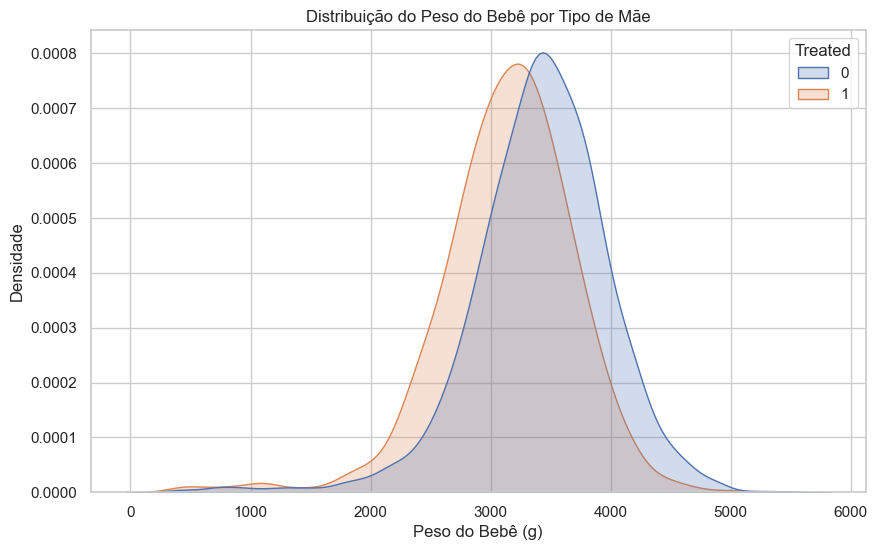
\includegraphics[width=0.5\linewidth,height=\textheight,keepaspectratio]{Fig.png}

}

\caption{\label{fig-distribution}Distribuição do peso dos bebês}

\end{figure}%

\section{Method}\label{method}

A relação pode ser representada pelas equações:

\[
Y = \alpha + \beta T + \gamma X + \epsilon
\]

\[
T = \alpha + \beta Z + \gamma X + \epsilon
\]

Explicar as variáveis, hipótese de identificação, fontes de viés e
justificativa da estratégia.

\section{Results}\label{results}

\begin{longtable}[]{@{}
  >{\raggedright\arraybackslash}p{(\linewidth - 12\tabcolsep) * \real{0.2258}}
  >{\raggedright\arraybackslash}p{(\linewidth - 12\tabcolsep) * \real{0.1452}}
  >{\raggedright\arraybackslash}p{(\linewidth - 12\tabcolsep) * \real{0.1774}}
  >{\raggedright\arraybackslash}p{(\linewidth - 12\tabcolsep) * \real{0.0968}}
  >{\raggedright\arraybackslash}p{(\linewidth - 12\tabcolsep) * \real{0.1129}}
  >{\raggedright\arraybackslash}p{(\linewidth - 12\tabcolsep) * \real{0.0645}}
  >{\raggedright\arraybackslash}p{(\linewidth - 12\tabcolsep) * \real{0.1774}}@{}}
\caption{Tabela de Resultados}\tabularnewline
\toprule\noalign{}
\begin{minipage}[b]{\linewidth}\raggedright
Modelo
\end{minipage} & \begin{minipage}[b]{\linewidth}\raggedright
Efeito
\end{minipage} & \begin{minipage}[b]{\linewidth}\raggedright
Erro-Padrão
\end{minipage} & \begin{minipage}[b]{\linewidth}\raggedright
T-test
\end{minipage} & \begin{minipage}[b]{\linewidth}\raggedright
P-valor
\end{minipage} & \begin{minipage}[b]{\linewidth}\raggedright
N
\end{minipage} & \begin{minipage}[b]{\linewidth}\raggedright
R² Ajustado
\end{minipage} \\
\midrule\noalign{}
\endfirsthead
\toprule\noalign{}
\begin{minipage}[b]{\linewidth}\raggedright
Modelo
\end{minipage} & \begin{minipage}[b]{\linewidth}\raggedright
Efeito
\end{minipage} & \begin{minipage}[b]{\linewidth}\raggedright
Erro-Padrão
\end{minipage} & \begin{minipage}[b]{\linewidth}\raggedright
T-test
\end{minipage} & \begin{minipage}[b]{\linewidth}\raggedright
P-valor
\end{minipage} & \begin{minipage}[b]{\linewidth}\raggedright
N
\end{minipage} & \begin{minipage}[b]{\linewidth}\raggedright
R² Ajustado
\end{minipage} \\
\midrule\noalign{}
\endhead
\bottomrule\noalign{}
\endlastfoot
Treated-Model1 & -275.2519 & 21.4528 & -12.83 & 0.0000 & 4642 &
0.0341 \\
Treated-Model2 & -218.1870 & 22.0917 & -9.88 & 0.0000 & 4642 & 0.0544 \\
Treated-Model3 & -203.0297 & 22.0547 & -9.21 & 0.0000 & 4642 & 0.0870 \\
\end{longtable}

\textbf{Notas:} Resultados estimados com variáveis de controle.

\section{Robustness Analysis}\label{robustness-analysis}

Apresentar placebo, métodos alternativos, diferentes amostras. Cada
parágrafo descreve uma análise de robustez e seus resultados.

\section{Discussion and Cost and Benefit
Analysis}\label{discussion-and-cost-and-benefit-analysis}

\subsection{Discussion}\label{discussion}

Interpretar os resultados, relacionar com mecanismos econômicos e
literatura. Explicar divergências com estudos anteriores. Explorar o
contexto econômico.

\begin{longtable}[]{@{}llllll@{}}
\caption{Cost and Benefit Analysis}\tabularnewline
\toprule\noalign{}
Política & Custo (R\$) & Juros (10\%) & Produção & Insumos & Receita \\
\midrule\noalign{}
\endfirsthead
\toprule\noalign{}
Política & Custo (R\$) & Juros (10\%) & Produção & Insumos & Receita \\
\midrule\noalign{}
\endhead
\bottomrule\noalign{}
\endlastfoot
A & 20 milhões & 2 milhões & 5 MW & 576 mil & 3,36 mi \\
B & 200 milhões & 20 milhões & 50 MW & 5,76 mi & 33,6 mi \\
C & 400 milhões & 40 milhões & 100 MW & 11,52 mi & 67,2 mi \\
D & 2 bilhões & 200 milhões & 500 MW & 57,6 mi & 336 mi \\
\end{longtable}

\section{Final Remarks}\label{final-remarks}

Reafirmar os principais resultados e sua relevância teórica e prática.
Discutir limitações da pesquisa e possibilidades futuras. Concluir
destacando a contribuição científica e as implicações políticas/sociais
dos achados.

\section{Referências}\label{referuxeancias}

As citações devem estar no formato Este método foi proposto por
\citet{hadash2018estimate}.


\bibliography{Refs.bib}



\end{document}
